\chapter{Harmonogram realizacji projektu}
\label{chap:Harmonogram realizacji projektu}

\begin{enumerate}
    \item \textbf{Dzień pierwszy}: Stworzenie podstawowej bazy danych oraz klasy \texttt{DatabaseConnector} oraz \texttt{Okno Bazowe}
    
    \item \textbf{Dzień drugi}: Ułożenie planu GUI, stworzenie takich klas jak \texttt{Walidacja}, \texttt{WygladPrzyciskow}, dodanie pakietu \texttt{Figures} oraz \texttt{logo.png}
    
    \item \textbf{Dzień trzeci}: Dodanie całego pakietu \texttt{serwis}
    
    \item \textbf{Dzień czwarty}: Dodanie \texttt{MenuGlowne} oraz zrobienie metody wywołania w \texttt{main}
    
    \item \textbf{Dzień piąty}: Dodanie \texttt{OknoLogowania}, \texttt{OknoRejestracji} oraz \texttt{PanelUzytkownika}
    
    \item \textbf{Dzień szósty}: Dodanie \texttt{PanelAdministratora}, ulepszenie kodów oraz bazy danych
    
    \item \textbf{Dzień siódmy}: Ostatnie poprawki i testy
    
    \item \textbf{Dzień ósmy}: Dokumentacja
\end{enumerate}

\begin{figure}[H]
    \centering
    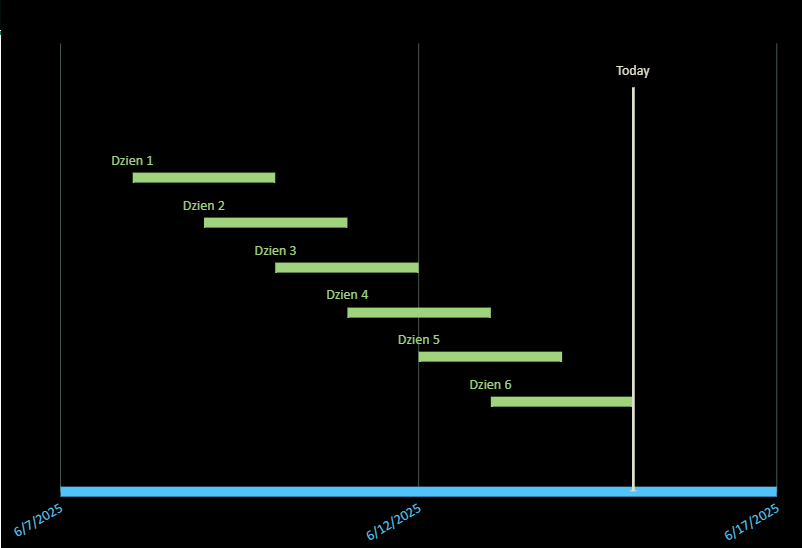
\includegraphics[width=.9\linewidth]{figures/SchematGrantta.png}\
    \caption{SchematGrantta.\label{SchematGrantta}}
\end{figure}

